\documentclass[11pt,a4paper]{article}
% allow both latex and PDFlatex compatibility  (from pdfTeX FAQ)
\usepackage{hyperlatex}

\usepackage{pifont}
\usepackage{amsmath}
\usepackage{amssymb}
%\usepackage{psfig}
\usepackage{array}
\usepackage{supertabular}
%\usepackage{fancyheadings}
\usepackage{here}
\usepackage{eepic,epic}
%\usepackage{pslatex} % devrait corriger le pb de fontes dans les pdfs mais le fichier produit n'est pas beau
\usepackage[english]{babel}
\usepackage{alltt}
% \usepackage{textcomp]


\texonly{\newcommand{\tilda}{{$_{\widetilde{\ }}$}}}
%\texonly{\newcommand{\tilda}{{\~{}}}}
\htmlonly{\newcommand{\tilda}{\verb+~+}}

\texonly{\usepackage{graphicx}
\usepackage{makeidx}
\usepackage[pdftex,pageanchor=true,hyperindex=true,pagebackref=true,pdfhighlight=/O,pdfauthor={Yves Renard}]{hyperref}%pour le pdf
\usepackage{xspace} % insere un espace si necessaire 
\usepackage{underscore}

\newcommand{\ds}{\displaystyle}
\oddsidemargin -0.9cm
\evensidemargin -0.9cm
\topmargin -1cm
\textheight 22.5cm
\textwidth 17.6cm
\headheight 1.0cm
}
\makeindex


\T \newcommand{\Reel}{{\rm I\hspace{-0.15em}R}}
\W \newcommand{\Reel}{\htmlsym{real}}
\T \newcommand{\ds}{\displaystyle}
\W \newcommand{\ds}{}
\newcommand{\Frac}[2]{{\ds \frac{\ds #1}{\ds #2}}}


% \W .. is equivalent to \htmlonly{..}
\W \newcommand{\HlxIcons}{./}
%\W \usepackage{frames} % navigation panel
\W \htmldirectory{getfem_project}
\W \htmlname{getfem_project}
\W \setcounter{htmldepth}{2}
\W \setcounter{htmlautomenu}{2}
\W \renewcommand{\HlxMeta}{\xml{META description="getfem++ user manual"}}
\htmlonly{%
  \htmlpanelfield{Index}{getfem_project}
  \htmlcss{docstyle.css}
  \newcommand{\text}[1]{\mathrm{#1}}
  \newcommand{\WEB}[2]{\xlink{#2}{#1}}
  \newcommand{\nabla}{\htmlsym{nabla}} % renamed \xmlent by lastest version of hyperlatex
  \newcommand{\ell}{\htmlsym{tau}}
  \newcommand{\lambda}{\htmlsym{lambda}}
  \newcommand{\varepsilon}{\htmlsym{epsilon}}
  \newcommand{\phi}{\htmlsym{phi}}
  \newcommand{\varphi}{\htmlsym{phi}}
  \newcommand{\psi}{\htmlsym{psi}}
  \newcommand{\sigma}{\htmlsym{sigma}}
  \newcommand{\nu}{\htmlsym{nu}}
  \newcommand{\beta}{\htmlsym{beta}}
  \newcommand{\gamma}{\htmlsym{gamma}}
  \newcommand{\alpha}{\htmlsym{alpha}}
  \newcommand{\Gamma}{\htmlsym{Gamma}}
  \newcommand{\Delta}{\htmlsym{Delta}}
  \newcommand{\delta}{\htmlsym{delta}}
  \newcommand{\Omega}{\htmlsym{Omega}}
  \newcommand{\omega}{\htmlsym{omega}}
  \newcommand{\tau}{\htmlsym{tau}}
  \newcommand{\partial}{\htmlsym{part}}
  \newcommand{\sum}{\htmlsym{sum}}
  \newcommand{\subset}{\htmlsym{sub}}
  \newcommand{\int}{{\Large\htmlsym{int}}}
}
\texonly{
  \newcommand{\WEB}[2]{\href{#1}{#2}}
}
\T \newcommand{\Div}{\textrm{div}}
\W \newcommand{\Div}{div}
\T \newcommand{\Grad}{\textrm{grad}}
\W \newcommand{\Grad}{grad}
\T \newcommand{\Rot}{\textrm{curl}}
\W \newcommand{\Rot}{curl}

\W \newcommand{\gf}{getfem++~}
\T \newcommand{\gf}{{\sc Getfem++}\xspace}

\W \newcommand{\newpage}{}
\W \newcommand{\hspace}[1]{ }
\W \newcommand{\left}{} % pour les left\(i\right) 
\W \newcommand{\right}{}
\W \newenvironment{alltt}{\begin{example}}{\end{example}}
\T \newenvironment{cppcode}{\begin{alltt}}{\end{alltt}}
\W \newenvironment{cppcode}{\begin{rawxml}<div class="cppcode">\end{rawxml}\begin{example}}{\end{example}\begin{rawxml}</div>\end{rawxml}}

\T \newcommand{\cpp}[1]{\texttt{#1}}
\T \newcommand{\filename}[1]{\texttt{#1}}

%doxfilename and doxref : used by doxygenlinks.tex
\T \newcommand{\doxfilename}[2]{\texttt{#1}}
\T \newcommand{\doxref}[2]{\cpp{#1}}

\W \newcommand{\cpp}[1]{\xmlattributes*{tt}{class="inlinecppcode"}\texttt{#1}}
\W \newcommand{\filename}[1]{\xmlattributes*{tt}{style="color:red"}\texttt{#1}}
\W \newcommand{\doxfilename}[2]{\xmlattributes*{tt}{class="inlinecppcode"}\texttt{\WEB{../getfem_reference/#2.html}{#1}}\xspace}
\W \newcommand{\doxref}[2]{\xmlattributes*{tt}{class="inlinecppcode"}\texttt{\WEB{../getfem_reference/#2.html}{#1}}\xspace}

\T \newenvironment{ctableau}[2]{\begin{center}\begin{supertabular}{#1}}{\end{supertabular}\end{center}}
\W \newenvironment{ctableau}[2]{\xmlattributes*{table}{border=1 align="center"}\begin{tabular}{#2}}{\end{tabular}}

\newcommand{\WEBB}[1]{\WEB{#1}{#1}}


% macros for linking filenames and classnames to the doxygen doc of getfem
% (i.e. \getfemmeshh \dalbitvector etc.) 
% edit updatedoxlinks.py to add new types/files
\newcommand{\getfemnormh}{\doxfilename{getfem/getfem\_norm.h}{getfem__norm_8h}}\xspace
\newcommand{\bgeotconvexstructureh}{\doxfilename{getfem/bgeot\_convex\_structure.h}{bgeot__convex__structure_8h}}\xspace
\newcommand{\getfemmeshregionh}{\doxfilename{getfem/getfem\_mesh\_region.h}{getfem__mesh__region_8h}}\xspace
\newcommand{\dalnamingsystemh}{\doxfilename{getfem/dal\_naming\_system.h}{dal__naming__system_8h}}\xspace
\newcommand{\getfemmeshimh}{\doxfilename{getfem/getfem\_mesh\_im.h}{getfem__mesh__im_8h}}\xspace
\newcommand{\getfemintegrationh}{\doxfilename{getfem/getfem\_integration.h}{getfem__integration_8h}}\xspace
\newcommand{\getfemfemh}{\doxfilename{getfem/getfem\_fem.h}{getfem__fem_8h}}\xspace
\newcommand{\bgeotpolyh}{\doxfilename{getfem/bgeot\_poly.h}{bgeot__poly_8h}}\xspace
\newcommand{\gmmmatrixh}{\doxfilename{gmm/gmm\_matrix.h}{gmm__matrix_8h}}\xspace
\newcommand{\bgeotcommainith}{\doxfilename{getfem/bgeot\_comma\_init.h}{bgeot__comma__init_8h}}\xspace
\newcommand{\bgeotconvexh}{\doxfilename{getfem/bgeot\_convex.h}{bgeot__convex_8h}}\xspace
\newcommand{\dalsharedptrh}{\doxfilename{getfem/dal\_shared\_ptr.h}{dal__shared__ptr_8h}}\xspace
\newcommand{\gmmsolverNewtonh}{\doxfilename{gmm/gmm\_solver\_Newton.h}{gmm__solver__Newton_8h}}\xspace
\newcommand{\gmmexcepth}{\doxfilename{gmm/gmm\_except.h}{gmm__except_8h}}\xspace
\newcommand{\bgeotconvexrefh}{\doxfilename{getfem/bgeot\_convex\_ref.h}{bgeot__convex__ref_8h}}\xspace
\newcommand{\getfemimporth}{\doxfilename{getfem/getfem\_import.h}{getfem__import_8h}}\xspace
\newcommand{\getfemmeshfemh}{\doxfilename{getfem/getfem\_mesh\_fem.h}{getfem__mesh__fem_8h}}\xspace
\newcommand{\gmmvectorh}{\doxfilename{gmm/gmm\_vector.h}{gmm__vector_8h}}\xspace
\newcommand{\getfemmesherh}{\doxfilename{getfem/getfem\_mesher.h}{getfem__mesher_8h}}\xspace
\newcommand{\bgeotkdtreeh}{\doxfilename{getfem/bgeot\_kdtree.h}{bgeot__kdtree_8h}}\xspace
\newcommand{\getfemmeshh}{\doxfilename{getfem/getfem\_mesh.h}{getfem__mesh_8h}}\xspace
\newcommand{\gmmalgobaseh}{\doxfilename{gmm/gmm\_algobase.h}{gmm__algobase_8h}}\xspace
\newcommand{\dalbasich}{\doxfilename{getfem/dal\_basic.h}{dal__basic_8h}}\xspace
\newcommand{\bgeotrtreeh}{\doxfilename{getfem/bgeot\_rtree.h}{bgeot__rtree_8h}}\xspace
\newcommand{\bgeotmeshstructureh}{\doxfilename{getfem/bgeot\_mesh\_structure.h}{bgeot__mesh__structure_8h}}\xspace
\newcommand{\bgeotvectorh}{\doxfilename{getfem/bgeot\_vector.h}{bgeot__vector_8h}}\xspace
\newcommand{\getfemlevelseth}{\doxfilename{getfem/getfem\_level\_set.h}{getfem__level__set_8h}}\xspace
\newcommand{\getfemmodelingh}{\doxfilename{getfem/getfem\_modeling.h}{getfem__modeling_8h}}\xspace
\newcommand{\bgeotsmallvectorh}{\doxfilename{getfem/bgeot\_small\_vector.h}{bgeot__small__vector_8h}}\xspace
\newcommand{\bgeottensorh}{\doxfilename{getfem/bgeot\_tensor.h}{bgeot__tensor_8h}}\xspace
\newcommand{\gmmblash}{\doxfilename{gmm/gmm\_blas.h}{gmm__blas_8h}}\xspace
\newcommand{\gmmdenseqrh}{\doxfilename{gmm/gmm\_dense\_qr.h}{gmm__dense__qr_8h}}\xspace
\newcommand{\bgeotgeometrictransh}{\doxfilename{getfem/bgeot\_geometric\_trans.h}{bgeot__geometric__trans_8h}}\xspace
\newcommand{\dalbitvectorh}{\doxfilename{getfem/dal\_bit\_vector.h}{dal__bit__vector_8h}}\xspace
\newcommand{\gmmiterh}{\doxfilename{gmm/gmm\_iter.h}{gmm__iter_8h}}\xspace
\newcommand{\gmmstdh}{\doxfilename{gmm/gmm\_std.h}{gmm__std_8h}}\xspace
\newcommand{\ftoolh}{\doxfilename{getfem/bgeot\_ftool.h}{bgeot__ftool_8h}}\xspace
\newcommand{\getfemimlisth}{\doxfilename{getfem/getfem\_im\_list.h}{getfem__im__list_8h}}\xspace
\newcommand{\bgeotsparsetensorsh}{\doxfilename{getfem/bgeot\_sparse\_tensors.h}{bgeot__sparse__tensors_8h}}\xspace
\newcommand{\getfemplasticityh}{\doxfilename{getfem/getfem\_plasticity.h}{getfem__plasticity_8h}}\xspace
\newcommand{\getfemmeshslicersh}{\doxfilename{getfem/getfem\_mesh\_slicers.h}{getfem__mesh__slicers_8h}}\xspace
\newcommand{\dalstaticstoredobjectsh}{\doxfilename{getfem/dal\_static\_stored\_objects.h}{dal__static__stored__objects_8h}}\xspace
\newcommand{\getfemexporth}{\doxfilename{getfem/getfem\_export.h}{getfem__export_8h}}\xspace
\newcommand{\getfemmatelemh}{\doxfilename{getfem/getfem\_mat\_elem.h}{getfem__mat__elem_8h}}\xspace
\newcommand{\getfemconfigh}{\doxfilename{getfem/getfem\_config.h}{getfem__config_8h}}\xspace
\newcommand{\getfemsuperluh}{\doxfilename{getfem/getfem\_superlu.h}{getfem__superlu_8h}}\xspace
\newcommand{\bgeotconfigh}{\doxfilename{getfem/bgeot\_config.h}{bgeot__config_8h}}\xspace
\newcommand{\gmmdefh}{\doxfilename{gmm/gmm\_def.h}{gmm__def_8h}}\xspace
\newcommand{\getfemmeshimlevelseth}{\doxfilename{getfem/getfem\_mesh\_im\_level\_set.h}{getfem__mesh__im__level__set_8h}}\xspace
\newcommand{\daltash}{\doxfilename{getfem/dal\_tas.h}{dal__tas_8h}}\xspace
\newcommand{\bgeotgeotransinvh}{\doxfilename{getfem/bgeot\_geotrans\_inv.h}{bgeot__geotrans__inv_8h}}\xspace
\newcommand{\gmmlapackinterfaceh}{\doxfilename{gmm/gmm\_lapack\_interface.h}{gmm__lapack__interface_8h}}\xspace
\newcommand{\gmmrefh}{\doxfilename{gmm/gmm\_ref.h}{gmm__ref_8h}}\xspace
\newcommand{\daltreesortedh}{\doxfilename{getfem/dal\_tree\_sorted.h}{dal__tree__sorted_8h}}\xspace
\newcommand{\getfemregularmeshesh}{\doxfilename{getfem/getfem\_regular\_meshes.h}{getfem__regular__meshes_8h}}\xspace
\newcommand{\getfemspiderfemh}{\doxfilename{getfem/getfem\_spider\_fem.h}{getfem__spider__fem_8h}}\xspace
\newcommand{\getfemderivativesh}{\doxfilename{getfem/getfem\_derivatives.h}{getfem__derivatives_8h}}\xspace
\newcommand{\getfemassemblingh}{\doxfilename{getfem/getfem\_assembling.h}{getfem__assembling_8h}}\xspace
\newcommand{\getfemXfemh}{\doxfilename{getfem/getfem\_Xfem.h}{getfem__Xfem_8h}}\xspace
\newcommand{\getfemmeshlevelseth}{\doxfilename{getfem/getfem\_mesh\_level\_set.h}{getfem__mesh__level__set_8h}}\xspace
\newcommand{\bgeotimbricatedboxh}{\doxfilename{getfem/bgeot\_imbricated\_box.h}{bgeot__imbricated__box_8h}}\xspace
\newcommand{\getfemCoulombfrictionh}{\doxfilename{getfem/getfem\_Coulomb\_friction.h}{getfem__Coulomb__friction_8h}}\xspace
\newcommand{\getfemcontexth}{\doxfilename{getfem/getfem\_context.h}{getfem__context_8h}}\xspace
\newcommand{\linkmsgh}{\doxfilename{getfem/getfem\_linkmsg.h}{getfem__linkmsg_8h}}\xspace
\newcommand{\getfemNavierStokesh}{\doxfilename{getfem/getfem\_Navier\_Stokes.h}{getfem__Navier__Stokes_8h}}\xspace
\newcommand{\dalbacktraceh}{\doxfilename{getfem/dal\_backtrace.h}{dal__backtrace_8h}}\xspace
\newcommand{\getfemassemblingtensorsh}{\doxfilename{getfem/getfem\_assembling\_tensors.h}{getfem__assembling__tensors_8h}}\xspace
\newcommand{\getfeminterpolatedfemoldh}{\doxfilename{getfem/getfem\_interpolated\_fem\_old.h}{getfem__interpolated__fem__old_8h}}\xspace
\newcommand{\getfemmeshsliceh}{\doxfilename{getfem/getfem\_mesh\_slice.h}{getfem__mesh__slice_8h}}\xspace
\newcommand{\getfemmatelemtypeh}{\doxfilename{getfem/getfem\_mat\_elem\_type.h}{getfem__mat__elem__type_8h}}\xspace
\newcommand{\getfemfemlevelseth}{\doxfilename{getfem/getfem\_fem\_level\_set.h}{getfem__fem__level__set_8h}}\xspace
\newcommand{\getfemexternaldatafemh}{\doxfilename{getfem/getfem\_external\_data\_fem.h}{getfem__external__data__fem_8h}}\xspace
\newcommand{\gmmprecondildlth}{\doxfilename{gmm/gmm\_precond\_ildlt.h}{gmm__precond__ildlt_8h}}\xspace
\newcommand{\bgeotpermutationsh}{\doxfilename{getfem/bgeot\_permutations.h}{bgeot__permutations_8h}}\xspace
\newcommand{\gmmh}{\doxfilename{gmm/gmm.h}{gmm_8h}}\xspace
\newcommand{\getfemfourthorderh}{\doxfilename{getfem/getfem\_fourth\_order.h}{getfem__fourth__order_8h}}\xspace
\newcommand{\gmmscaledh}{\doxfilename{gmm\_scaled.h}{gmm/gmm__scaled_8h}}\xspace
\newcommand{\gmmkernelh}{\doxfilename{gmm\_kernel.h}{gmm/gmm__kernel_8h}}\xspace
\newcommand{\getfeminterpolatedfemh}{\doxfilename{getfem/getfem\_interpolated\_fem.h}{getfem__interpolated__fem_8h}}\xspace
\newcommand{\gmmMUMPSinterfaceh}{\doxfilename{gmm\_MUMPS\_interface.h}{gmm/gmm__MUMPS__interface_8h}}\xspace
\newcommand{\bgeotmeshh}{\doxfilename{getfem/bgeot\_mesh.h}{bgeot__mesh_8h}}\xspace
\newcommand{\getfemerrorestimateh}{\doxfilename{getfem/getfem\_error\_estimate.h}{getfem__error__estimate_8h}}\xspace
\newcommand{\getfemmeshfemsumh}{\doxfilename{getfem/getfem\_mesh\_fem\_sum.h}{getfem__mesh__fem__sum_8h}}\xspace
\newcommand{\getfemmodelsolversh}{\doxfilename{getfem/getfem\_model\_solvers.h}{getfem__model__solvers_8h}}\xspace
\newcommand{\gmmconditionnumberh}{\doxfilename{gmm\_condition\_number.h}{gmm__condition__number_8h}}\xspace
\newcommand{\getfemnonlinearelasticityh}{\doxfilename{getfem/getfem\_nonlinear\_elasticity.h}{getfem__nonlinear__elasticity_8h}}\xspace
\newcommand{\gmmtrisolveh}{\doxfilename{gmm/gmm\_tri\_solve.h}{gmm__tri__solve_8h}}\xspace
\newcommand{\getfemlinearizedplatesh}{\doxfilename{getfem/getfem\_linearized\_plates.h}{getfem__linearized__plates_8h}}\xspace
\newcommand{\getfemmeshfemlevelseth}{\doxfilename{getfem/getfem\_mesh\_fem\_level\_set.h}{getfem__mesh__fem__level__set_8h}}\xspace
\newcommand{\getfeminterpolationh}{\doxfilename{getfem/getfem\_interpolation.h}{getfem__interpolation_8h}}\xspace
\newcommand{\getfemmeshfemproducth}{\doxfilename{getfem/getfem\_mesh\_fem\_product.h}{getfem__mesh__fem__product_8h}}\xspace
\newcommand{\bgeotpolycompositeh}{\doxfilename{getfem/bgeot\_poly\_composite.h}{bgeot__poly__composite_8h}}\xspace
\newcommand{\gmmconjugatedh}{\doxfilename{gmm/gmm\_conjugated.h}{gmm__conjugated_8h}}\xspace
\newcommand{\gmmsolverSchwarzadditiveh}{\doxfilename{gmm/gmm\_solver\_Schwarz\_additive.h}{gmm__solver__Schwarz__additive_8h}}\xspace
\newcommand{\gmminoutputh}{\doxfilename{gmm/gmm\_inoutput.h}{gmm__inoutput_8h}}\xspace
\newcommand{\gmmdenseluh}{\doxfilename{gmm/gmm\_dense\_lu.h}{gmm__dense__lu_8h}}\xspace
\newcommand{\gmmsolvercgh}{\doxfilename{gmm/gmm\_solver\_cg.h}{gmm__solver__cg_8h}}\xspace
\newcommand{\gmmsuperluinterfaceh}{\doxfilename{gmm/gmm\_superlu\_interface.h}{gmm__superlu__interface_8h}}\xspace
\newcommand{\dalsingletonh}{\doxfilename{getfem/dal\_singleton.h}{dal__singleton_8h}}\xspace
\newcommand{\getfemgausslobattofemcoefh}{\doxfilename{getfem/getfem\_gauss\_lobatto\_fem\_coef.h}{getfem__gauss__lobatto__fem__coef_8h}}\xspace
\newcommand{\gmmdenseHouseholderh}{\doxfilename{gmm/gmm\_dense\_Householder.h}{gmm__dense__Householder_8h}}\xspace
\newcommand{\gmmsolverqmrh}{\doxfilename{gmm/gmm\_solver\_qmr.h}{gmm__solver__qmr_8h}}\xspace
\newcommand{\gmmopth}{\doxfilename{gmm/gmm\_opt.h}{gmm__opt_8h}}\xspace
\newcommand{\gmmvectortomatrixh}{\doxfilename{gmm/gmm\_vector\_to\_matrix.h}{gmm__vector__to__matrix_8h}}\xspace
\newcommand{\gmminterfacebgeoth}{\doxfilename{gmm/gmm\_interface\_bgeot.h}{gmm__interface__bgeot_8h}}\xspace
\newcommand{\getfemmeshfemglobalfunctionh}{\doxfilename{getfem/getfem\_mesh\_fem\_global\_function.h}{getfem__mesh__fem__global__function_8h}}\xspace
\newcommand{\gmmsolverconstrainedcgh}{\doxfilename{gmm/gmm\_solver\_constrained\_cg.h}{gmm__solver__constrained__cg_8h}}\xspace
\newcommand{\gmmsolvergmresh}{\doxfilename{gmm/gmm\_solver\_gmres.h}{gmm__solver__gmres_8h}}\xspace
\newcommand{\gmmdensesylvesterh}{\doxfilename{gmm/gmm\_dense\_sylvester.h}{gmm__dense__sylvester_8h}}\xspace
\newcommand{\gmminterfaceh}{\doxfilename{gmm/gmm\_interface.h}{gmm__interface_8h}}\xspace
\newcommand{\gmmdomaindecomph}{\doxfilename{gmm/gmm\_domain\_decomp.h}{gmm__domain__decomp_8h}}\xspace
\newcommand{\gmmsolveridgmresh}{\doxfilename{gmm/gmm\_solver\_idgmres.h}{gmm__solver__idgmres_8h}}\xspace
\newcommand{\gmmsubindexh}{\doxfilename{gmm/gmm\_sub\_index.h}{gmm__sub__index_8h}}\xspace
\newcommand{\gmmsolverbicgstabh}{\doxfilename{gmm/gmm\_solver\_bicgstab.h}{gmm__solver__bicgstab_8h}}\xspace
\newcommand{\gmmitersolversh}{\doxfilename{gmm/gmm\_iter\_solvers.h}{gmm__iter__solvers_8h}}\xspace
\newcommand{\gmmsubvectorh}{\doxfilename{gmm/gmm\_sub\_vector.h}{gmm__sub__vector_8h}}\xspace
\newcommand{\gmmprecondh}{\doxfilename{gmm/gmm\_precond.h}{gmm__precond_8h}}\xspace
\newcommand{\gmmmodifiedgramschmidth}{\doxfilename{gmm/gmm\_modified\_gram\_schmidt.h}{gmm__modified__gram__schmidt_8h}}\xspace
\newcommand{\gmmrealparth}{\doxfilename{gmm/gmm\_real\_part.h}{gmm__real__part_8h}}\xspace
\newcommand{\gmmsubmatrixh}{\doxfilename{gmm/gmm\_sub\_matrix.h}{gmm__sub__matrix_8h}}\xspace
\newcommand{\gmmpreconddiagonalh}{\doxfilename{gmm/gmm\_precond\_diagonal.h}{gmm__precond__diagonal_8h}}\xspace
\newcommand{\gmmprecondiluh}{\doxfilename{gmm/gmm\_precond\_ilu.h}{gmm__precond__ilu_8h}}\xspace
\newcommand{\gmmprecondiluth}{\doxfilename{gmm/gmm\_precond\_ilut.h}{gmm__precond__ilut_8h}}\xspace
\newcommand{\gmmprecondmrapproxinverseh}{\doxfilename{gmm/gmm\_precond\_mr\_approx\_inverse.h}{gmm__precond__mr__approx__inverse_8h}}\xspace
\newcommand{\getfemnonlinearelasticitytwoh}{\doxfilename{getfem/getfem\_nonlinear\_elasticity2.h}{getfem__nonlinear__elasticity2_8h}}\xspace
\newcommand{\gmmtransposedh}{\doxfilename{gmm/gmm\_transposed.h}{gmm__transposed_8h}}\xspace
\newcommand{\gmmprecondildltth}{\doxfilename{gmm/gmm\_precond\_ildltt.h}{gmm__precond__ildltt_8h}}\xspace
\newcommand{\gmmprecondilutph}{\doxfilename{gmm/gmm\_precond\_ilutp.h}{gmm__precond__ilutp_8h}}\xspace
\newcommand{\gmmblasinterfaceh}{\doxfilename{gmm/gmm\_blas\_interface.h}{gmm__blas__interface_8h}}\xspace
\newcommand{\gmmsolverbfgsh}{\doxfilename{gmm/gmm\_solver\_bfgs.h}{gmm__solver__bfgs_8h}}\xspace
\newcommand{\bgeotconvexrefsimplexifiedcc}{\doxfilename{getfem/bgeot\_convex\_ref\_simplexified.cc}{bgeot__convex__ref__simplexified_8cc}}\xspace
\newcommand{\getfemmeshfemlevelsetcc}{\doxfilename{getfem/getfem\_mesh\_fem\_level\_set.cc}{getfem__mesh__fem__level__set_8cc}}\xspace
\newcommand{\getfemlevelsetcc}{\doxfilename{getfem/getfem\_level\_set.cc}{getfem__level__set_8cc}}\xspace
\newcommand{\getfemexportcc}{\doxfilename{getfem/getfem\_export.cc}{getfem__export_8cc}}\xspace
\newcommand{\getfemmatelemcc}{\doxfilename{getfem/getfem\_mat\_elem.cc}{getfem__mat__elem_8cc}}\xspace
\newcommand{\ftoolcc}{\doxfilename{getfem/bgeot\_ftool.cc}{bgeot__ftool_8cc}}\xspace
\newcommand{\getfemmeshercc}{\doxfilename{getfem/getfem\_mesher.cc}{getfem__mesher_8cc}}\xspace
\newcommand{\bgeotgeometrictranscc}{\doxfilename{getfem/bgeot\_geometric\_trans.cc}{bgeot__geometric__trans_8cc}}\xspace
\newcommand{\getfemerrorestimatecc}{\doxfilename{getfem/getfem\_error\_estimate.cc}{getfem__error__estimate_8cc}}\xspace
\newcommand{\getfemfemcc}{\doxfilename{getfem/getfem\_fem.cc}{getfem__fem_8cc}}\xspace
\newcommand{\getfemimportcc}{\doxfilename{getfem/getfem\_import.cc}{getfem__import_8cc}}\xspace
\newcommand{\getfemmeshlevelsetcc}{\doxfilename{getfem/getfem\_mesh\_level\_set.cc}{getfem__mesh__level__set_8cc}}\xspace
\newcommand{\getfemfemlevelsetcc}{\doxfilename{getfem/getfem\_fem\_level\_set.cc}{getfem__fem__level__set_8cc}}\xspace
\newcommand{\getfemmodelingcc}{\doxfilename{getfem/getfem\_modeling.cc}{getfem__modeling_8cc}}\xspace
\newcommand{\getfemassemblingtensorscc}{\doxfilename{getfem/getfem\_assembling\_tensors.cc}{getfem__assembling__tensors_8cc}}\xspace
\newcommand{\getfemmeshfemcc}{\doxfilename{getfem/getfem\_mesh\_fem.cc}{getfem__mesh__fem_8cc}}\xspace
\newcommand{\dalstaticstoredobjectscc}{\doxfilename{getfem/dal\_static\_stored\_objects.cc}{dal__static__stored__objects_8cc}}\xspace
\newcommand{\getfemmeshimlevelsetcc}{\doxfilename{getfem/getfem\_mesh\_im\_level\_set.cc}{getfem__mesh__im__level__set_8cc}}\xspace
\newcommand{\getfemmeshfemsumcc}{\doxfilename{getfem/getfem\_mesh\_fem\_sum.cc}{getfem__mesh__fem__sum_8cc}}\xspace
\newcommand{\getfemmeshimcc}{\doxfilename{getfem/getfem\_mesh\_im.cc}{getfem__mesh__im_8cc}}\xspace
\newcommand{\bgeotpolycc}{\doxfilename{getfem/bgeot\_poly.cc}{bgeot__poly_8cc}}\xspace
\newcommand{\getfemmeshcc}{\doxfilename{getfem/getfem\_mesh.cc}{getfem__mesh_8cc}}\xspace
\newcommand{\getfemmatelemtypecc}{\doxfilename{getfem/getfem\_mat\_elem\_type.cc}{getfem__mat__elem__type_8cc}}\xspace
\newcommand{\bgeotconvexrefcc}{\doxfilename{getfem/bgeot\_convex\_ref.cc}{bgeot__convex__ref_8cc}}\xspace
\newcommand{\getfeminterpolatedfemoldcc}{\doxfilename{getfem/getfem\_interpolated\_fem\_old.cc}{getfem__interpolated__fem__old_8cc}}\xspace
\newcommand{\getfemintegrationcc}{\doxfilename{getfem/getfem\_integration.cc}{getfem__integration_8cc}}\xspace
\newcommand{\getfemmeshslicerscc}{\doxfilename{getfem/getfem\_mesh\_slicers.cc}{getfem__mesh__slicers_8cc}}\xspace
\newcommand{\bgeotpolycompositecc}{\doxfilename{getfem/bgeot\_poly\_composite.cc}{bgeot__poly__composite_8cc}}\xspace
\newcommand{\getfemregularmeshescc}{\doxfilename{getfem/getfem\_regular\_meshes.cc}{getfem__regular__meshes_8cc}}\xspace
\newcommand{\getfemmeshfemproductcc}{\doxfilename{getfem/getfem\_mesh\_fem\_product.cc}{getfem__mesh__fem__product_8cc}}\xspace
\newcommand{\getfeminterpolatedfemcc}{\doxfilename{getfem/getfem\_interpolated\_fem.cc}{getfem__interpolated__fem_8cc}}\xspace
\newcommand{\getfemmeshregioncc}{\doxfilename{getfem/getfem\_mesh\_region.cc}{getfem__mesh__region_8cc}}\xspace
\newcommand{\getfemmeshfemglobalfunctioncc}{\doxfilename{getfem/getfem\_mesh\_fem\_global\_function.cc}{getfem__mesh__fem__global__function_8cc}}\xspace
\newcommand{\getfemsuperlucc}{\doxfilename{getfem/getfem\_superlu.cc}{getfem__superlu_8cc}}\xspace
\newcommand{\getfemnonlinearelasticitycc}{\doxfilename{getfem/getfem\_nonlinear\_elasticity.cc}{getfem__nonlinear__elasticity_8cc}}\xspace
\newcommand{\dalbitvectorcc}{\doxfilename{getfem/dal\_bit\_vector.cc}{dal__bit__vector_8cc}}\xspace
\newcommand{\bgeotsparsetensorscc}{\doxfilename{getfem/bgeot\_sparse\_tensors.cc}{bgeot__sparse__tensors_8cc}}\xspace
\newcommand{\getfemcontextcc}{\doxfilename{getfem/getfem\_context.cc}{getfem__context_8cc}}\xspace
\newcommand{\bgeotmeshstructurecc}{\doxfilename{getfem/bgeot\_mesh\_structure.cc}{bgeot__mesh__structure_8cc}}\xspace
\newcommand{\getfemXfemcc}{\doxfilename{getfem/getfem\_Xfem.cc}{getfem__Xfem_8cc}}\xspace
\newcommand{\bgeotgeotransinvcc}{\doxfilename{getfem/bgeot\_geotrans\_inv.cc}{bgeot__geotrans__inv_8cc}}\xspace
\newcommand{\getfemintegrationcompositecc}{\doxfilename{getfem/getfem\_integration\_composite.cc}{getfem__integration__composite_8cc}}\xspace
\newcommand{\bgeotrtreecc}{\doxfilename{getfem/bgeot\_rtree.cc}{bgeot__rtree_8cc}}\xspace
\newcommand{\dalbacktracecc}{\doxfilename{getfem/dal\_backtrace.cc}{dal__backtrace_8cc}}\xspace
\newcommand{\bgeotconvexstructurecc}{\doxfilename{getfem/bgeot\_convex\_structure.cc}{bgeot__convex__structure_8cc}}\xspace
\newcommand{\bgeotimbricatedboxcc}{\doxfilename{getfem/bgeot\_imbricated\_box.cc}{bgeot__imbricated__box_8cc}}\xspace
\newcommand{\bgeotkdtreecc}{\doxfilename{getfem/bgeot\_kdtree.cc}{bgeot__kdtree_8cc}}\xspace
\newcommand{\bgeotsmallvectorcc}{\doxfilename{getfem/bgeot\_small\_vector.cc}{bgeot__small__vector_8cc}}\xspace
\newcommand{\dalsingletoncc}{\doxfilename{getfem/dal\_singleton.cc}{dal__singleton_8cc}}\xspace
\newcommand{\getfeminterpolationcc}{\doxfilename{getfem/getfem\_interpolation.cc}{getfem__interpolation_8cc}}\xspace
\newcommand{\getfemmeshslicecc}{\doxfilename{getfem/getfem\_mesh\_slice.cc}{getfem__mesh__slice_8cc}}\xspace
\newcommand{\getfemfemcompositecc}{\doxfilename{getfem/getfem\_fem\_composite.cc}{getfem__fem__composite_8cc}}\xspace
\newcommand{\dalbitvector}{\doxref{dal::bit\_vector}{classdal_1_1bit__vector}}\xspace
\newcommand{\dalbvvisitor}{\doxref{dal::bv\_visitor}{classdal_1_1bv__visitor}}\xspace
\newcommand{\bgeotconvexstructure}{\doxref{bgeot::convex\_structure}{classbgeot_1_1convex__structure}}\xspace
\newcommand{\bgeotpconvexstructure}{\doxref{bgeot::pconvex\_structure}{classbgeot_1_1convex__structure}}\xspace
\newcommand{\bgeotconvexref}{\doxref{bgeot::convex\_ref}{classbgeot_1_1convex__ref}}\xspace
\newcommand{\bgeotpconvexref}{\doxref{bgeot::pconvex\_ref}{classbgeot_1_1convex__ref}}\xspace
\newcommand{\bgeotgeometrictrans}{\doxref{bgeot::geometric\_trans}{classbgeot_1_1geometric__trans}}\xspace
\newcommand{\bgeotpgeometrictrans}{\doxref{bgeot::pgeometric\_trans}{classbgeot_1_1geometric__trans}}\xspace
\newcommand{\getfemvirtualfem}{\doxref{getfem::virtual\_fem}{classgetfem_1_1virtual__fem}}\xspace
\newcommand{\getfempfem}{\doxref{getfem::pfem}{classgetfem_1_1virtual__fem}}\xspace
\newcommand{\getfemmesh}{\doxref{getfem::mesh}{classgetfem_1_1mesh}}\xspace
\newcommand{\getfemmeshregion}{\doxref{getfem::mesh\_region}{classgetfem_1_1mesh__region}}\xspace
\newcommand{\getfemmrvisitor}{\doxref{getfem::mr\_visitor}{classgetfem_1_1mr__visitor}}\xspace
\newcommand{\bgeotmeshstructure}{\doxref{bgeot::mesh\_structure}{classbgeot_1_1mesh__structure}}\xspace
\newcommand{\getfemgenericassembly}{\doxref{getfem::generic\_assembly}{classgetfem_1_1generic__assembly}}\xspace
\newcommand{\getfemmeshim}{\doxref{getfem::mesh\_im}{classgetfem_1_1mesh__im}}\xspace
\newcommand{\getfemmeshfem}{\doxref{getfem::mesh\_fem}{classgetfem_1_1mesh__fem}}\xspace
\newcommand{\getfemstoredmeshslice}{\doxref{getfem::stored\_mesh\_slice}{classgetfem_1_1stored__mesh__slice}}\xspace
\newcommand{\getfemsliceraction}{\doxref{getfem::slicer\_action}{classgetfem_1_1slicer__action}}\xspace
\newcommand{\getfemmeshslicecvdofdatabase}{\doxref{getfem::mesh\_slice\_cv\_dof\_data\_base}{classgetfem_1_1mesh__slice__cv__dof__data__base}}\xspace
\newcommand{\getfemslicernone}{\doxref{getfem::slicer\_none}{classgetfem_1_1slicer__none}}\xspace
\newcommand{\getfemslicerboundary}{\doxref{getfem::slicer\_boundary}{classgetfem_1_1slicer__boundary}}\xspace
\newcommand{\getfemslicerapplydeformation}{\doxref{getfem::slicer\_apply\_deformation}{classgetfem_1_1slicer__apply__deformation}}\xspace
\newcommand{\getfemslicerhalfspace}{\doxref{getfem::slicer\_half\_space}{classgetfem_1_1slicer__half__space}}\xspace
\newcommand{\getfemslicersphere}{\doxref{getfem::slicer\_sphere}{classgetfem_1_1slicer__sphere}}\xspace
\newcommand{\getfemslicercylinder}{\doxref{getfem::slicer\_cylinder}{classgetfem_1_1slicer__cylinder}}\xspace
\newcommand{\getfemslicerisovalues}{\doxref{getfem::slicer\_isovalues}{classgetfem_1_1slicer__isovalues}}\xspace
\newcommand{\getfemslicermeshwithmesh}{\doxref{getfem::slicer\_mesh\_with\_mesh}{classgetfem_1_1slicer__mesh__with__mesh}}\xspace
\newcommand{\getfemslicerunion}{\doxref{getfem::slicer\_union}{classgetfem_1_1slicer__union}}\xspace
\newcommand{\getfemslicerintersect}{\doxref{getfem::slicer\_intersect}{classgetfem_1_1slicer__intersect}}\xspace
\newcommand{\getfemslicercomplementary}{\doxref{getfem::slicer\_complementary}{classgetfem_1_1slicer__complementary}}\xspace
\newcommand{\getfemslicerbuildmesh}{\doxref{getfem::slicer\_build\_mesh}{classgetfem_1_1slicer__build__mesh}}\xspace
\newcommand{\getfemslicerbuildedgesmesh}{\doxref{getfem::slicer\_build\_edges\_mesh}{classgetfem_1_1slicer__build__edges__mesh}}\xspace
\newcommand{\getfemslicerbuildstoredmeshslice}{\doxref{getfem::slicer\_build\_stored\_mesh\_slice}{classgetfem_1_1slicer__build__stored__mesh__slice}}\xspace
\newcommand{\getfemslicerexplode}{\doxref{getfem::slicer\_explode}{classgetfem_1_1slicer__explode}}\xspace
\newcommand{\getfemmeshslicer}{\doxref{getfem::mesh\_slicer}{classgetfem_1_1mesh__slicer}}\xspace
\newcommand{\getfemdxexport}{\doxref{getfem::dx\_export}{classgetfem_1_1dx__export}}\xspace
\newcommand{\getfemvtkexport}{\doxref{getfem::vtk\_export}{classgetfem_1_1vtk__export}}\xspace
\newcommand{\getfemlevelset}{\doxref{getfem::level\_set}{classgetfem_1_1level__set}}\xspace
\newcommand{\getfemmeshlevelset}{\doxref{getfem::mesh\_level\_set}{classgetfem_1_1mesh__level__set}}\xspace
\newcommand{\getfemmeshimlevelset}{\doxref{getfem::mesh\_im\_level\_set}{classgetfem_1_1mesh__im__level__set}}\xspace
\newcommand{\getfemmeshfemlevelset}{\doxref{getfem::mesh\_fem\_level\_set}{classgetfem_1_1mesh__fem__level__set}}\xspace
\newcommand{\getfemmodelstate}{\doxref{getfem::model\_state}{classgetfem_1_1model__state}}\xspace
\newcommand{\getfemmdbrickabstractcommonbase}{\doxref{getfem::mdbrick\_abstract\_common\_base}{classgetfem_1_1mdbrick__abstract__common__base}}\xspace
\newcommand{\getfemmdbrickabstract}{\doxref{getfem::mdbrick\_abstract}{classgetfem_1_1mdbrick__abstract}}\xspace
\newcommand{\getfemmdbrickparameter}{\doxref{getfem::mdbrick\_parameter}{classgetfem_1_1mdbrick__parameter}}\xspace
\newcommand{\getfemmdbrickabstractlinearpde}{\doxref{getfem::mdbrick\_abstract\_linear\_pde}{classgetfem_1_1mdbrick__abstract__linear__pde}}\xspace
\newcommand{\getfemmdbrickgenericelliptic}{\doxref{getfem::mdbrick\_generic\_elliptic}{classgetfem_1_1mdbrick__generic__elliptic}}\xspace
\newcommand{\getfemmdbricksourceterm}{\doxref{getfem::mdbrick\_source\_term}{classgetfem_1_1mdbrick__source__term}}\xspace
\newcommand{\getfemmdbrickconstraint}{\doxref{getfem::mdbrick\_constraint}{classgetfem_1_1mdbrick__constraint}}\xspace
\newcommand{\getfemmdbrickDirichlet}{\doxref{getfem::mdbrick\_Dirichlet}{classgetfem_1_1mdbrick__Dirichlet}}\xspace
\newcommand{\getfemmdbrickisotropiclinearizedelasticity}{\doxref{getfem::mdbrick\_isotropic\_linearized\_elasticity}{classgetfem_1_1mdbrick__isotropic__linearized__elasticity}}\xspace
\newcommand{\getfemmdbrickQUterm}{\doxref{getfem::mdbrick\_QU\_term}{classgetfem_1_1mdbrick__QU__term}}\xspace
\newcommand{\getfemmdbricklinearincomp}{\doxref{getfem::mdbrick\_linear\_incomp}{classgetfem_1_1mdbrick__linear__incomp}}\xspace
\newcommand{\getfemmdbrickplasticity}{\doxref{getfem::mdbrick\_plasticity}{classgetfem_1_1mdbrick__plasticity}}\xspace
\newcommand{\getfemmdbrickisotropiclinearizedplate}{\doxref{getfem::mdbrick\_isotropic\_linearized\_plate}{classgetfem_1_1mdbrick__isotropic__linearized__plate}}\xspace
\newcommand{\getfemmdbrickmixedisotropiclinearizedplate}{\doxref{getfem::mdbrick\_mixed\_isotropic\_linearized\_plate}{classgetfem_1_1mdbrick__mixed__isotropic__linearized__plate}}\xspace
\newcommand{\getfemmdbrickplatesourceterm}{\doxref{getfem::mdbrick\_plate\_source\_term}{classgetfem_1_1mdbrick__plate__source__term}}\xspace
\newcommand{\getfemmdbrickplatesimplesupport}{\doxref{getfem::mdbrick\_plate\_simple\_support}{classgetfem_1_1mdbrick__plate__simple__support}}\xspace
\newcommand{\getfemmdbrickplateclampedsupport}{\doxref{getfem::mdbrick\_plate\_clamped\_support}{classgetfem_1_1mdbrick__plate__clamped__support}}\xspace
\newcommand{\getfemmdbrickplateclosing}{\doxref{getfem::mdbrick\_plate\_closing}{classgetfem_1_1mdbrick__plate__closing}}\xspace
\newcommand{\getfemmdbricknonlinearelasticity}{\doxref{getfem::mdbrick\_nonlinear\_elasticity}{classgetfem_1_1mdbrick__nonlinear__elasticity}}\xspace
\newcommand{\getfemmdbricknonlinearincomp}{\doxref{getfem::mdbrick\_nonlinear\_incomp}{classgetfem_1_1mdbrick__nonlinear__incomp}}\xspace
\newcommand{\getfemabstracthyperelasticlaw}{\doxref{getfem::abstract\_hyperelastic\_law}{structgetfem_1_1abstract__hyperelastic__law}}\xspace
\newcommand{\getfemSaintVenantKirchhoffhyperelasticlaw}{\doxref{getfem::SaintVenant\_Kirchhoff\_hyperelastic\_law}{structgetfem_1_1SaintVenant__Kirchhoff__hyperelastic__law}}\xspace
\newcommand{\getfemCiarletGeymonathyperelasticlaw}{\doxref{getfem::Ciarlet\_Geymonat\_hyperelastic\_law}{structgetfem_1_1Ciarlet__Geymonat__hyperelastic__law}}\xspace
\newcommand{\getfemMooneyRivlinhyperelasticlaw}{\doxref{getfem::Mooney\_Rivlin\_hyperelastic\_law}{structgetfem_1_1Mooney__Rivlin__hyperelastic__law}}\xspace
\newcommand{\gmmiteration}{\doxref{gmm::iteration}{classgmm_1_1iteration}}\xspace




\begin{document}
\htmltitle{Getfem Project}
\htmlpanel{0}%disable navigation panel

\begin{center}
\texonly{
  
\includegraphics[width=10cm,angle=0]{logogetfemwhitebg}\\[0.2cm]
  a Generic Finite Element library in C++ \\[0.5cm]
  {\LARGE Documentation, part \Huge 1} \\[0.5cm]
  \fbox{\Huge \sc Description of the project} \\[0.5cm]
  { \large Yves {\sc Renard}, Julien {\sc Pommier} \footnote{ \it ICJ - CNRS UMR 5208, INSA de Lyon, 20, rue Albert Einstein, 69621 Villeurbanne Cedex, FRANCE, Yves.Renard@insa-lyon.fr } } \\[1.0cm]
  \today \\[1.0cm]
}
\htmlonly{
  \xlink{\htmlimg{logogetfem.png}{The Getfem++ logo}}{http://home.gna.org/getfem/}\\[2cm]
  a Generic Finite Element library in C++ \par\par
  {\LARGE Documentation, part \Huge 1} \\ \par\par
  {\Huge Description of the project } \\ \par
  { \large \xlink{Yves Renard}{mailto:Yves.Renard@insa-lyon.fr}, \xlink{Julien Pommier}{mailto:Julien.Pommier@insa-toulouse.fr}}\\
  {\it ICJ - CNRS UMR 5208, INSA de Lyon, 20, rue Albert Einstein, 69621 Villeurbanne Cedex, FRANCE.}\\
  \today \par\par
}
\end{center}

% \begin{abstract}
% Basic user documentation for \gf .
% \end{abstract}
\htmlonly{\\\\\\}
\texonly{~\\[4cm]}
\begin{quote}
Copyright (C) 2000-2020 Yves Renard, Julien Pommier.\\
The program GetFEM is free software; you can redistribute it and/or modify
it under the terms of the GNU Lesser General Public License as published by
the Free Software Foundation; either version 3 of the License, or
(at your option) any later version along with the GCC Runtime Library
Exception either version 3.1 or (at your option) any later version.
This program is distributed in the hope that it will be useful,
but WITHOUT ANY WARRANTY; without even the implied warranty of
MERCHANTABILITY or FITNESS FOR A PARTICULAR PURPOSE.  See the
GNU Lesser General Public License for more details.
You should have received a copy of the GNU  Lesser General Public License
along with this program; if not, write to the Free Software Foundation,
Inc., 51 Franklin Street, Fifth Floor, Boston, MA  02110-1301  USA
\end{quote}

\newpage

%%%%%%%%%%%%%%%%%%%%%%%%%%%%%%%%%%%%%%%%%%%%%%%%%%%%%%%%%%%%%%%%%%%%%%%%%
%          INTRODUCTION                                                 %
%%%%%%%%%%%%%%%%%%%%%%%%%%%%%%%%%%%%%%%%%%%%%%%%%%%%%%%%%%%%%%%%%%%%%%%%%

\section{Introduction}

The \gf project focuses on the development of a generic finite element library.
The goal is to provide a finite element framework which allows to easily build  numerical code for the modelisation of system described by partial differential equations (p.d.e.). A special attention is paid to the flexibility of the use of the library in the sense that the switch from a method offered by the library to another is made as easy as possible.

The major point allowing this compared to traditional finite element codes is the complete separation between the description of p.d.e. models and finite element methods. Moreover, a separation is made between integration methods (exact or approximated), geometric transformations (linear or not) and finite element methods of arbitrary degrees described on a reference element. \gf can be used to build very general finite elements codes, where the finite elements, integration methods, dimension of the meshes, are just some parameters that can be changed very easily, thus allowing a large spectrum of experimentations. Numerous examples are available in the \filename{tests} directory of the distribution.

The goal is also to make the addition of new finite element method as simple as possible. For standard method, a description of the finite element shape functions and the type of connection of degrees of freedom on the reference element is sufficient. Extensions are provided for Hermite elements, piecewise polynomial, non-polynomial and vectorial elements, XFem. Examples of predefined available methods are Pk on simplices in arbitrary degrees and dimensions, Qk on parallelepipeds, P1, P2 with bubble functions, Hermite elements, elements with hierarchic basis (for multigrid methods for instance), discontinuous Pk or Qk, XFem, Argyris, HCT, Raviart-Thomas.

The library also includes the usual tools for finite elements such as assembly procedures for classical PDEs, interpolation methods, computation of norms, mesh operations, boundary conditions, post-processing tools such as extraction of slices from a mesh ...

\gf has no meshing capabilities (apart regular meshes, and a not exploitable attempt), hence, in many situations, it is necessary to import meshes. Imports formats currently known by getfem are GiD , GmSH and emc2 mesh files. However, given a mesh, it is possible to refine it automatically.

The aim of the \gf project is not to provide a ready to use finite element code allowing for instance structural mechanics computations with a graphic interface. It is basically a library allowing the build of C++ finite element codes. However, the matlab and python interfaces allows to easily build application coupling the definition of the problem, the finite element methods selection and the graphical post-processing.

The future of the project is to continue to develop the finite element framework, focusing on the following points.
\begin{itemize}
  \item Background consolidation of the existing modules (with a reflection on the optimal representation of meshes, degrees of freedom, finite element methods ...).
  \item Developpement of innovating methods.
  \item Reflection on the optimal way to represent complex p.d.e. models with the maximum of flexibility and reusability. The brick system is a first step in this direction.
\end{itemize}


\newpage
\tableofcontents
\newpage

\section{Global structure of the library}

This section describes the diagram of the different modules of the \gf library.
The current state and perspective for each module is described in section \ref{sec:descmod}.


\begin{figure}[H]
  \begin{center}
    \texonly{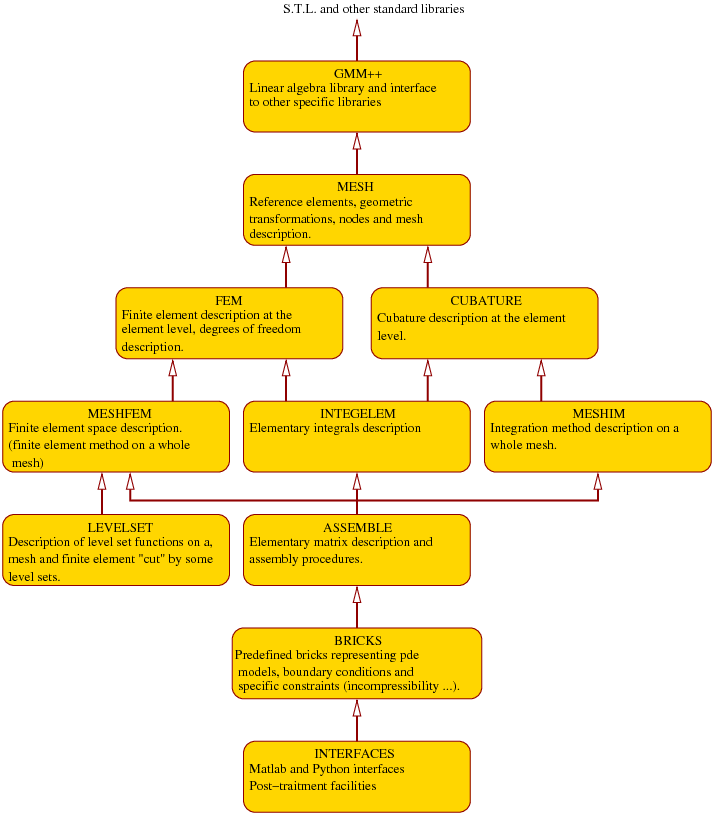
\includegraphics[width=0.9\linewidth,angle=0]{diagram.pdf}}
    \htmlonly{\htmlimg{diagram.png}{Diagram of \gf}}
  \end{center}
  \caption{ \it Diagram of \gf }
  \label{fig:elemf}
\end{figure}

\newpage



\section{Introduction to the fem description in \gf}


\subsection{Convex structures}

Finite element methods are defined on small convex domains called elements. The simplest element on which a finite element method can be defined is a segment (simplex of dimension 1), other possibilities are triangles, tetrahedrons (simplices of dimension 2 and 3), prisms, parallelepiped ...
In \gf, a type of element (for us, a convex) is described by the object \cpp{bgeot::convex\_structure} defined in the file \cpp{bgeot\_convex\_structure.h}.\\[0.5cm]
It describes only the structure of the convex not the coordinates of the vertices.
This structure is not to be manipulated by itself, because it is not necessary that more than one structure of this type describe the same type of convex. What will be manipulated is a pointer on such a descriptor which has to be declared with the type \cpp{bgeot::pconvex\_structure} \\ \\

The following functions give a pointer onto the descriptor of the usual type of elements:

\begin{center} \begin{ctableau}{|m{0.45\linewidth}|m{0.5\linewidth}|}{ll} \hline
 \cpp{bgeot::simplex\_structure(dim\_type d)} & description of a simplex of dimension \cpp{d}. \\ \hline
 \cpp{bgeot::parallelepiped\_structure(dim\_type\;d)} &  description of a parallelepiped of dimension \cpp{d}. \\ \hline
 \cpp{bgeot::convex\_product\_structure( bgeot::pconvex\_structure p1, bgeot::pconvex\_structure p2) } & description of the direct product of \cpp{p1} and \cpp{p2}.\\ \hline
 \cpp{bgeot::prism\_structure(dim\_type d)}  & description of a prism of dimension \cpp{d}\\ \hline
\end{ctableau} \end{center}

For instance if one needs the description of a square, one can call equivalently\\
\cpp{p = bgeot::parallelepiped\_structure(2); }
or\\
\cpp{p = bgeot::convex\_product\_structure(bgeot::simplex\_structure(1),\\        ~ \hspace{18.5em} bgeot::simplex\_structure(1)); }\\

The descriptor contains in particular  the number of faces (\cpp{p->nb\_faces()}), the dimension of the convex (\cpp{p->dim()}), for the number of vertices (\cpp{p->nb\_points()}). Other information is the number of vertices of each face, the description of a face and the eventual reference to a more basic description (used for the description of geometric transformations).

\htmlonly{\label{fig:elem}}
\begin{figure}[H]
  \begin{center}
    \texonly{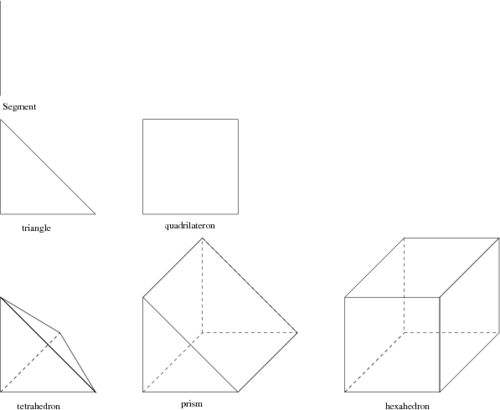
\includegraphics[width=10cm]{getfemelemelem.pdf}}
    \htmlonly{\htmlimg{getfemelemelem.png}{usual elements}}
  \end{center}
  \caption{ \it Usual elements. }
  \texonly{\label{fig:elem}}
\end{figure}


\subsection{Convexes of reference}

A convex of reference is a particular real element, i.e. a structure of convex with a list of vertices. It describes the particular element from which a finite element method is defined. In the file \cpp{bgeot\_convex\_ref.h} the object\\[0.5cm]
\cpp{bgeot::convex\_of\_reference }\\[0.5cm]
makes this description. The library keeps only one  description for each type of convex. So what will be manipulated is a pointer of type \cpp{bgeot::pconvex\_ref } on the descriptor\\[0.5cm]

The following functions build the descriptions:

\begin{center} \begin{ctableau}{|m{0.55\linewidth}|m{0.4\linewidth}|}{ll} \hline
\cpp{bgeot::simplex\_of\_reference(dim\_type d)} & description of the simplex of reference of dimension \cpp{d} \\ \hline
  
  \cpp{bgeot::simplex\_of\_reference(dim\_type d, short\_type k)} & description of the simplex of reference of dimension \cpp{d} with degree \cpp{k} Lagrange grid. \\ \hline

  \cpp{bgeot::convex\_ref\_product(pconvex\_ref a, pconvex\_ref b)} & description of the direct product of two convexes of reference.\\ \hline
  
  \cpp{bgeot::parallelepiped\_of\_reference(dim\_type\;d)} & description of the parallelepiped of reference of dimension \cpp{d}  \\ \hline
\end{ctableau} \end{center}

The vertices correspond to the classical vertices for such reference element. For instance the vertices for the triangle are $(0, 0), (1, 0)$ and $(0, 1)$. It corresponds to the configuration shown in Figure \ref{fig:elem}

If \cpp{p} is of type \cpp{bgeot::pconvex\_ref } then \cpp{p->structure()} is the corresponding convex structure. Thus for instance \cpp{p->structure()->nb\_points()} gives the number of vertices. The function \cpp{p->points()} give the array of vertices and \cpp{p->points()[0]} is the first vertex. The function \cpp{p->is\_in(const base\_node \&pt)} return a real which is negative if the point \cpp{pt} is in the element. The function \cpp{p->is\_in\_face(short\_type f, const base\_node \&pt)} return a real which is null if the point \cpp{pt} is in the face \cpp{k} of the element. Other functions can be found in \cpp{bgeot\_convex\_ref.h} and \cpp{bgeot\_convex.h}.

\subsection{Shape function type}

Most of the time the shape functions of finite element methods are polynomials, at least on the convex of reference. But, the possibility is given to have other types of elements. It is possible to define other kind of base functions such as piecewise polynomials, interpolant wavelets ...\\
To be used by the finite element description, a shape function type must be able to be evaluated on a point (\cpp{a = F.eval(pt)}, where \cpp{pt} is a \cpp{base\_node}) and must have a method to compute the derivtive with respect to the ith variable (\cpp{F.derivative(i)}).

For the moment, only polynomials and piecewise polynomials are defined in the files \cpp{bgeot\_poly.h} and \cpp{bgeot\_poly\_composite.h}


\subsection{Geometric transformations}

\begin{figure}[htb]
  \begin{center}
    \texonly{\includegraphics[width=10cm]{getfemelemtrans.pdf}}
    \htmlonly{\htmlimg{getfemelemtrans.png}{usual elements}}
  \end{center}
  \caption{ \it Geometric transformation }
  \label{fig:transgeo}
\end{figure}

A geometric transformation is a polynomial application\\
\begin{center} $ \tau : T' \subset \Reel^P \longrightarrow T \subset\Reel^N, $ \end{center}
which maps the reference element $T'$ to the real element $T$.
The geometric nodes are denoted
\begin{center} $ g^i, \ \ i = 0 .. n_g - 1. $ \end{center}
The geometric transformation is described thanks to a $n_g$ components polynomial vector (In fact, as an extention, non polynomial geometric transformation can also be supported by Getfem++, but this is very rarely used).
\begin{center} ${\cal N}(x'), $ \end{center}
such that
\begin{center} $ \ds \tau(x') = \sum_{i = 0}^{n_g - 1} {\cal N}_i(x') g^i.$\end{center}
Denoting
\begin{center} $ G = (g^0; g^1; ...; g^{n_g - 1}), $ \end{center}
the $N \times n_g$ matrix containing of all the geometric nodes, one has
\begin{center} $ \texonly{\fbox}{$\hspace{1em}\tau(x') = G {\cal N}(x').\hspace{1em}$} $ \end{center}
The derivative of $\tau$ is then
\begin{center} $ \texonly{\fbox}{$\hspace{1em} K(x') := \nabla \tau(x') = G \nabla {\cal N}(x'),\hspace{1em}$} $ \end{center}
where $K(x') = \nabla \tau(x')$ is a $N \times P$ matrix and $\nabla {\cal N}(x')$ a $n_g \times P$ matrix.
The (transposed) pseudo-inverse of $\nabla\tau(x')$ is a $N\times P$ matrix denoted $B(x')$:
\begin{center} \texonly{$\fbox}{$\hspace{1em} B(x') := K(x')(K(x')^T K(x'))^{-1},\hspace{1em}$} \texonly{$} \end{center}
Of course, when $P=N$, one has $B(x')=K(x')^{-T}$.

Pointers on a descriptor of a geometric transformation can be obtained by the following function defined in the file \cpp{bgeot\_geometric\_trans.h}:\\[0.5cm]
\cpp{bgeot::pgeometric\_trans pgt = bgeot::geometric\_trans\_descriptor("name of trans"); }\\[0.5cm]
where \cpp{"name of trans"} can be chosen among the following list.
\begin{center} \begin{ctableau}{|m{0.3\linewidth}|m{0.65\linewidth}|}{ll} \hline
\cpp{"GT\_PK(n,k)"} & Description of the simplex transformation of dimension \cpp{n} and degree \cpp{k} (Most of the time, the degree 1 is used).\\ \hline
\cpp{"GT\_QK(n,k)"} & Description of the parallelepiped transformation of dimension \cpp{n} and degree \cpp{k}.\\ \hline
\cpp{"GT\_PRISM(n,k)"} & Description of the prism transformation of dimension \cpp{n} and degree \cpp{k}. \\ \hline
\cpp{"GT\_PRODUCT(a,b)"} & Description of the direct product of the two transformations \cpp{a} and \cpp{b}.\\ \hline
\cpp{"GT\_LINEAR\_PRODUCT(a,b)"} & Description of the direct product of the two transformations \cpp{a} and \cpp{b} keeping a linear transformation (this is a restriction of he previous function). This allows, for instance, to use exact integrations on regular meshes with parallelograms.\\ \hline
\end{ctableau} \end{center}

\subsection{Finite element methods description}

A finite element method is defined on a reference element $T' \subset \Reel^P$ by a set of $n_d$ nodes $a^i$ and corresponding base functions 
\begin{center}$ \varphi' ^i : T' \subset \Reel^P \longrightarrow \Reel^Q,$\end{center}
Denoting
\begin{center}$ \psi^i(x) = \varphi' ^i(x') = \varphi' ^i(\tau^{-1}(x)), $\end{center}
a supplementary linear transformation is allowed for the real base function
\begin{center}$ \varphi^i(x) = \sum_{j = 0}^{n_d - 1} M_{ij} \psi^j(x), $\end{center}
where $M$ is a $n_d \times n_d$ matrix possibly depending on the geometric transformation (i.e. on the real element). For basic elements as Lagrange elements this matrix is the identity matrix (it is simply ignored). In this case, we will say that the element is $\tau$-equivalent. This approach allows to define hermite elements (Argyris for instance) in a generic way, even with non linear transformations (i.e. mainly for curved boundaries).
We denote $[\varphi'(x')]$ the $n_d \times Q$ matrix whose ith line is $\varphi' ^i(x')$. Whis this notation, for a function is defined by 
\begin{center}$ f(x) = \sum_{i = 0}^{n_d - 1} \alpha_i \varphi^i(x), $\end{center}
one has
\begin{center} \texonly{$ \fbox}{$\hspace{1em} f(\tau(x')) = \alpha^T M [\varphi'(x')],\hspace{1em}$} \texonly{$}\end{center}
where $\alpha$ is the vector whose ith component is $\alpha_i$.

A certain number of description of classical finite element method are defined in the file \cpp{getfem\_fem.h}. See Appendix A for an exhaustive list of available finite element methods.\\

A pointer to the finite element descriptor of a method is obtained using the function\\[0.5cm]
{\tt getfem::pfem pfe = getfem::fem\_descriptor("name of method"); }\\[0.5cm]
We refer to the file {\tt getfem\_fem.C} for how to define a new finite element method.

\subsection{Volume integral} (to be annexed ?)
One has
\begin{center} $ \int_T f(x) dx = \int_{T'} f'(x') |\text{vol}\left(\Frac{\partial \tau(x')}{\partial x'_0} ;\Frac{\partial \tau(x')}{\partial x'_1}; ...; \Frac{\partial \tau(x')}{\partial x'_{P-1} }\right)| dx'. $\end{center}
Denoting $J_{\tau}(x')$ the jacobian
\begin{center} \texonly{$ \fbox}{$\hspace{1em} J_{\tau}(x') := |\text{vol}\left(\Frac{\partial \tau(x')}{\partial x'_0} ;\Frac{\partial \tau(x')}{\partial x'_1}; ...; \Frac{\partial \tau(x')}{\partial x'_{P-1} }\right)| = (\mbox{det}(K(x')^T K(x')))^{1/2},\hspace{1em}$} \texonly{$}\end{center}
one finally has
\begin{center} \texonly{$ \fbox}{$\hspace{1em} \ds \int_T f(x) dx = \int_{T'} f'(x')  J_{\tau}(x')dx'.\hspace{1em}$} \texonly{$} \end{center}
When $P = N$, the expression of the jacobian reduces to $J_{\tau}(x') = |\mbox{det}(K(x'))|$.

\subsection{Surface integral}
With $\Gamma$ a part of the boundary of $T$ a real element and $\Gamma'$ the corresponding boundary on the reference element $T'$, one has
\begin{center} \texonly{$ \fbox}{$\hspace{1em} \ds \int_{\Gamma} f(x) d\sigma = \int_{\Gamma'} f'(x') \|B(x'){\mathbf n'}\| J_{\tau}(x') d\sigma',\hspace{1em}$} \texonly{$} \end{center}
where ${\mathbf n}'$ is the unit normal to $T'$ on $\Gamma'$. In a same way
\begin{center} \texonly{$ \fbox}{$\hspace{1em} \ds \int_{\Gamma} F(x).{\mathbf n} d\sigma = \int_{\Gamma'} F'(x').(B(x'){\mathbf n}') J_{\tau}(x') d\sigma'.\hspace{1em}$} \texonly{$} \end{center}

\subsection{Derivative computation}
One has
\begin{center} $ \nabla f(x) = B(x') \nabla'\,f'(x'). $ \end{center}
\subsection{Second derivative computation}
Denoting 
\begin{center}$ \nabla^2 f = ({\Frac{\partial^2 f}{\partial x_i \partial x_j}})_{ij}, $  \end{center}
the $N \times N$ matrix and
\begin{center}$ X'(x') = \sum_{k = 0}^{N-1} \nabla'^2 \tau_k(x') \Frac{\partial f}{\partial x_k}(x) = \sum_{k = 0}^{N-1} \sum_{i = 0}^{P-1} \nabla'^2 \tau_k(x') B_{ki} \Frac{\partial f'}{\partial x'_i}(x'), $  \end{center}
the $P \times P$ matrix, then
\begin{center}$ \nabla'^2 f'(x') = X'(x') + K(x')^T \nabla^2 f(x) K(x'), $ \end{center}
and thus
\begin{center}$ \nabla^2 f(x) = B(x') (\nabla'^2 f'(x') - X'(x')) B(x')^T. $ \end{center}

In order to have uniform methods for the computation of elementary matrices, the Hessian is computed as a column vector $H f$ whose components are $\Frac{\partial^2 f}{\partial x^2_0}, {\Frac{\partial^2 f}{\partial x_1 \partial x_0}}, ... {\Frac{\partial^2 f}{\partial x^2_{N-1}}}$.
Then, with $B_2$ the $P^2 \times P$ matrix defined as
\begin{center} $ (B_2(x'))_{ij} = \sum_{k = 0}^{N-1} \Frac{\partial^2 \tau_k(x')}{\partial x'_{i / P} \partial x'_{i \mbox{ mod } P} } B_{kj}(x'), $\end{center}
and $B_3$ the $N^2 \times P^2$ matrix defined as
\begin{center} $ (B_3(x'))_{ij} = B_{i / N, j / P}(x') B_{i \mbox{ mod } N, j \mbox{ mod } P}(x'), $\end{center}
one has
\begin{center} \texonly{$ \fbox}{ $H f(x) = B_3(x') \left(H'\,f'(x') - B_2(x')\nabla'\,f'(x')\right). $} \texonly{$} \end{center}

\subsection{Example of elementary matrix} \label{elmminst}

Assume one needs to compute the elementary ``matrix'':
\begin{center} $ t(i_0, i_1, ..., i_7) = \int_{T} \varphi_{i_1}^{i_0}\; \partial_{i_4} \varphi_{i_3}^{i_2}\; \partial^2_{i_7 / P, i_7 \mbox{ mod } P} \varphi_{i_6}^{i_5} dx, $  \end{center}
The computations to be made on the reference elements are
\begin{center} $ t'_0(i_0, i_1, ..., i_7) = \int_{T'} \varphi'_{i_1}^{i_0}\; \partial_{i_4} \varphi'_{i_3}^{i_2}\; \partial^2_{i_7 / P, i_7 \mbox{ mod } P} \varphi'_{i_6}^{i_5}  J(x') dx', $ \end{center}
and
\begin{center} $ t'_1(i_0, i_1, ..., i_7) = \int_{T'} \varphi'_{i_1}^{i_0}\; \partial_{i_4} \varphi'_{i_3}^{i_2}\; \partial_{i_7} \varphi'_{i_6}^{i_5}  J(x') dx', $ \end{center}
Those two tensor can be computed once on the whole reference element if the geometric transformation is linear (because $J(x')$ is constant). If the geometric transformation is non-linear, what has to be stored is the value on each integration point. To compute the integral on the real element a certain number of reductions have to be made:
\begin{itemize}
    \item Concerning the first term ($\varphi_{i_1}^{i_0}$) nothing.
    \item Concerning the second term ($\partial_{i_4} \varphi_{i_3}^{i_2}$) a reduction with respect to $i_4$ with the matrix $B$.
    \item Concerning the third term ($\partial^2_{i_7 / P, i_7 \mbox{ mod } P} \varphi_{i_6}^{i_5}$) a reduction of $t'_0$ with respect to $i_7$ with the matrix $B_3$ and a reduction of $t'_1$ with respect also to $i_7$ with the matrix $B_3B_2$
 \end{itemize}
 The reductions are to be made on each integration point if the geometric transformation is non-linear. Once those reductions are done, an addition of all the tensor resulting of those reductions is made (with a factor equal to the load of each integration point if the geometric transformation is non-linear).

 If the finite element is non-$\tau$-equivalent, a supplementary reduction of the resulting tensor with the matrix $M$ has to be made.


















\section{Description of the different parts of the library} \label{sec:descmod}

\subsection{Gmm++ library}

\subsection{Mesh module}

\subsection{FEM module}

\subsection{CUBATURE module}

\subsection{MESHFEM module}

\subsection{MESHIM module}

\subsection{INTEGELEM module}

\subsection{ASSEMBLE module}

\subsection{BRICK module}

\subsection{Matlab and Python interfaces}




\section{Global perspectives of structuration, consolidation and growth}


\section{Appendix A, finite element method list}

\subsection{Dof codification}

\section{Appendix B, cubature method list}



\begin{thebibliography}{99}
% \bibliographystyle{apalike}
% \bibliographystyle{plain}
% \bibliography{all}

\bibitem{ciarlet1978}
  P.G.. {\texonly{\sc} Ciarlet},
  {\it The finite element method for elliptic problems}, Studies in Mathematics and its Applications vol. 4, North-Holland, 1978.

\bibitem{bank1983}
  R.E. {\texonly{\sc} Bank, A.H. Sherman, A. Weiser}
  {\it Refinement algorithms and data structures for regular local mesh refinement},
  in Scientific Computing IMACS, Amsterdam, North-Holland, pp 3-17, 1983

\bibitem{EncyclopCubature}
  R. {\texonly{\sc} Cools}
  {\it An Encyclopaedia of Cubature Formulas}, J. Complexity, \cpp{http://www.cs.kuleuven.ac.be/\tilda ines/research/ecf/ecf.html}
  
\bibitem{Xfem}
  N. {\texonly{\sc} Mo�s, J. Dolbow and T. Belytschko}
  {\it A finite element method for crack growth without remeshing },
  Int. J. Num. Meth. Engng. 46, 131-150 (1999).  

\bibitem{dh-to1984} 
  {\texonly{\sc} G. Dhatt, and  G. Touzot}
  {\it The Finite Element Method Displayed}, 
  J. Wiley \& Sons,  New York, 1984.



\end{thebibliography}

% \W \section*{Index}
% \texorhtml{\printindex}{\label{gfmindex}\htmlprintindex}

\end{document}
